\section{ROS Communication between RaspberryPi and Teensy }
\section{Obstacle Avoidance using Tangent Bug Algorithm}
Before this project begins with complex implementations of SLAM it first aims to prove that the robot can avoid obstacles on a predetermined path. For this obstacle the Tangent bug algorithm is used.\\

The tangent bug algorithm is designed for robots which have a finite sensor range such as the RPLIDAr-A1 (limited to 12 meters) and its algorithm is as follows:\\

\noindent \textbf{while} true do:\\
\tab \textbf{repeat}\\
\tab \tab Continuously move toward the point n in {T, Oi} which minimizes \\
\tab \tab d(x,n)+d(x, q-goal)\\
\tab \textbf{until}\\
\tab \tab The goal is encountered, \textbf{OR}\\
\tab \tab The direction that minimizes  d(x,n)+d(x, q-goal) begins to increase.\\
\\
\tab Chose a boundary following direction which continues in the same direction as the\\ 
\tab most recent motion-to-goal direction.\\
\\
\tab \textbf{repeat}\\
\tab \tab Continuously update d-reach, d-followed, and {Oi}\\
\tab \tab Continuously move toward the point n in {Oi} which is in the chosen boundary\\
\tab \tab direction\\
\tab \textbf{until}\\
\tab \tab The goal is reached \textbf{OR}\\
\tab \tab The robot completes a cycle around the obstacle in which case the goal cannot\\
\tab \tab be reached \textbf{OR}\\
\tab \tab d-reach < d-followed\\



\begin{figure}[H]
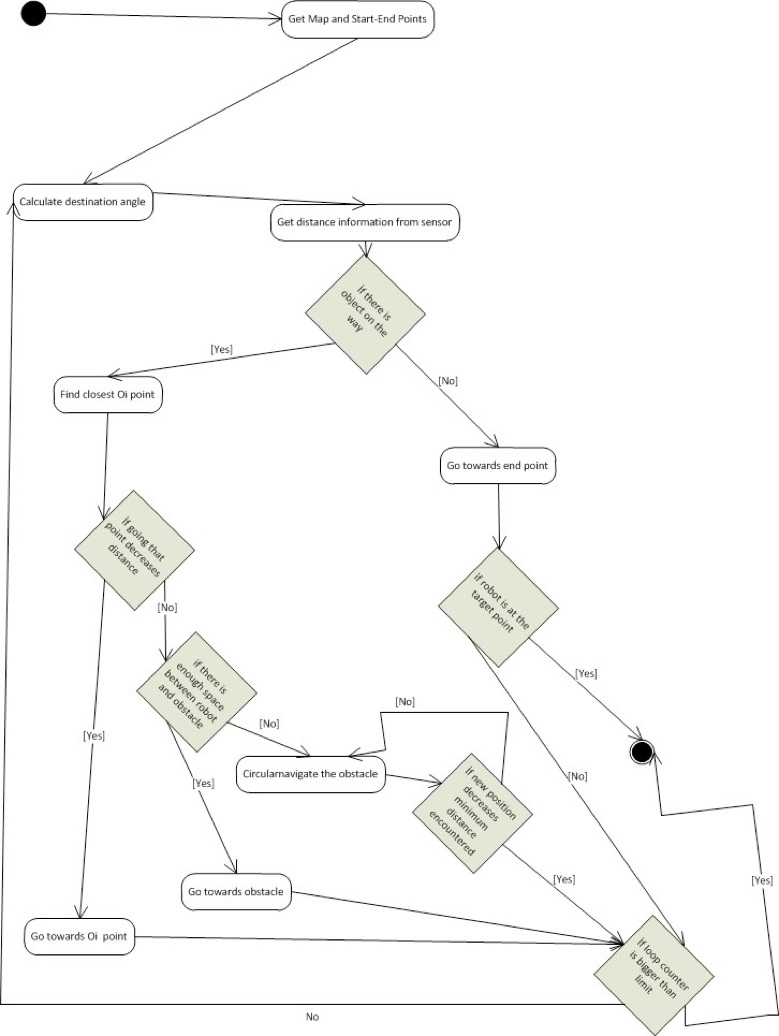
\includegraphics[width=\textwidth]{Figures/tangent_bug_diagram.jpg}
\centering
\caption{Flowchart of the tangent bug algorithm. Image courtesy of \cite{tangent_bug}}
\label{figure:infinite_corridor}
\end{figure}

\section{Mapping}
\section{EKF}
\section{Path Planning}
